\documentclass[a4paper,12pt]{article}
\usepackage{xcolor}
\usepackage{amsmath,amsfonts,amssymb}
\usepackage{geometry}
\usepackage{fancyhdr}
\usepackage{graphicx}
\usepackage{titlesec}
\usepackage{tikz}
\usepackage{booktabs}
\usepackage{array}
\usetikzlibrary{shadows}
\usepackage{tcolorbox}
\usepackage{float}
\usepackage{lipsum}
\usepackage{mdframed}
\usepackage{pagecolor}
\usepackage{mathpazo}   % Palatino font (serif)
\usepackage{microtype}  % Better typography

% Page background color
\pagecolor{gray!10!white}

% Geometry settings
\geometry{margin=0.5in}
\pagestyle{fancy}
\fancyhf{}

% Fancy header and footer
\fancyhead[C]{\textbf{\color{blue!80}CS754 Assignment-2}}
% \fancyhead[R]{\color{blue!80}Saksham Rathi}
\fancyfoot[C]{\thepage}

% Custom Section Color and Format with Sans-serif font
\titleformat{\section}
{\sffamily\color{purple!90!black}\normalfont\Large\bfseries}
{\thesection}{1em}{}

% Custom subsection format
\titleformat{\subsection}
{\sffamily\color{cyan!80!black}\normalfont\large\bfseries}
{\thesubsection}{1em}{}

% Stylish Title with TikZ (Enhanced with gradient)
\newcommand{\cooltitle}[1]{%
  \begin{tikzpicture}
    \node[fill=blue!20,rounded corners=10pt,inner sep=12pt, drop shadow, top color=blue!50, bottom color=blue!30] (box)
    {\Huge \bfseries \color{black} #1};
  \end{tikzpicture}
}
\usepackage{float} % Add this package

\newenvironment{solution}[2][]{%
    \begin{mdframed}[linecolor=blue!70!black, linewidth=2pt, roundcorner=10pt, backgroundcolor=yellow!10!white, skipabove=12pt, skipbelow=12pt]%
        \textbf{\large #2}
        \par\noindent\rule{\textwidth}{0.4pt}
}{
    \end{mdframed}
}

% Document title
\title{\cooltitle{CS754 Assignment-2}}
\author{{\bf Saksham Rathi, Ekansh Ravi Shankar, Kshitij Vaidya}}
\date{}

\begin{document}
\maketitle
\textbf{Declaration:} The work submitted is our own, and
we have adhered to the principles of academic honesty while completing and submitting this work. We have not referred to any unauthorized sources, and we have not used generative AI tools for the work submitted here.

\section*{Question 2}

\begin{solution}{Implementation of ISTA}
  We implement the Iterative Soft Thresholding Algorithm (ISTA) for solving the LASSO problem which is given by:
  \begin{equation}
    \min_{x} \frac{1}{2} \|Ax - b\|_2^2 + \lambda \|x\|_1
  \end{equation}
  \noindent where $A \in \mathbb{R}^{m \times n}$ is the product of the sensing matrix and the DCT basis matrix, $b \in \mathbb{R}^m$, $x \in \mathbb{R}^n$ and $\lambda > 0$ is the regularization parameter. The algorithm also requires us to decide on the step size $\alpha$ and the number of iterations to run the algorithm for. The constant $\alpha$ is taken as the maximum eigenvalue of $A^TA$ and the number of iterations is taken as 1000. 

  \begin{equation}
    \alpha = \max(\text{eig}(A^TA))
  \end{equation}

  \noindent Before running the algorithm on the \textbf{barbara.png}, we add some Gaussian Noise to the image and also normalise the cells of the image to be in the range $[0, 1]$. We then divide the image into overlapping patches of size $8 \times 8$ and run the ISTA algorithm on each patch. We then reconstruct the image from the patches and display the reconstructed image. The results are shown below:

\end{solution}

\begin{figure}[!htbp]
  \centering
  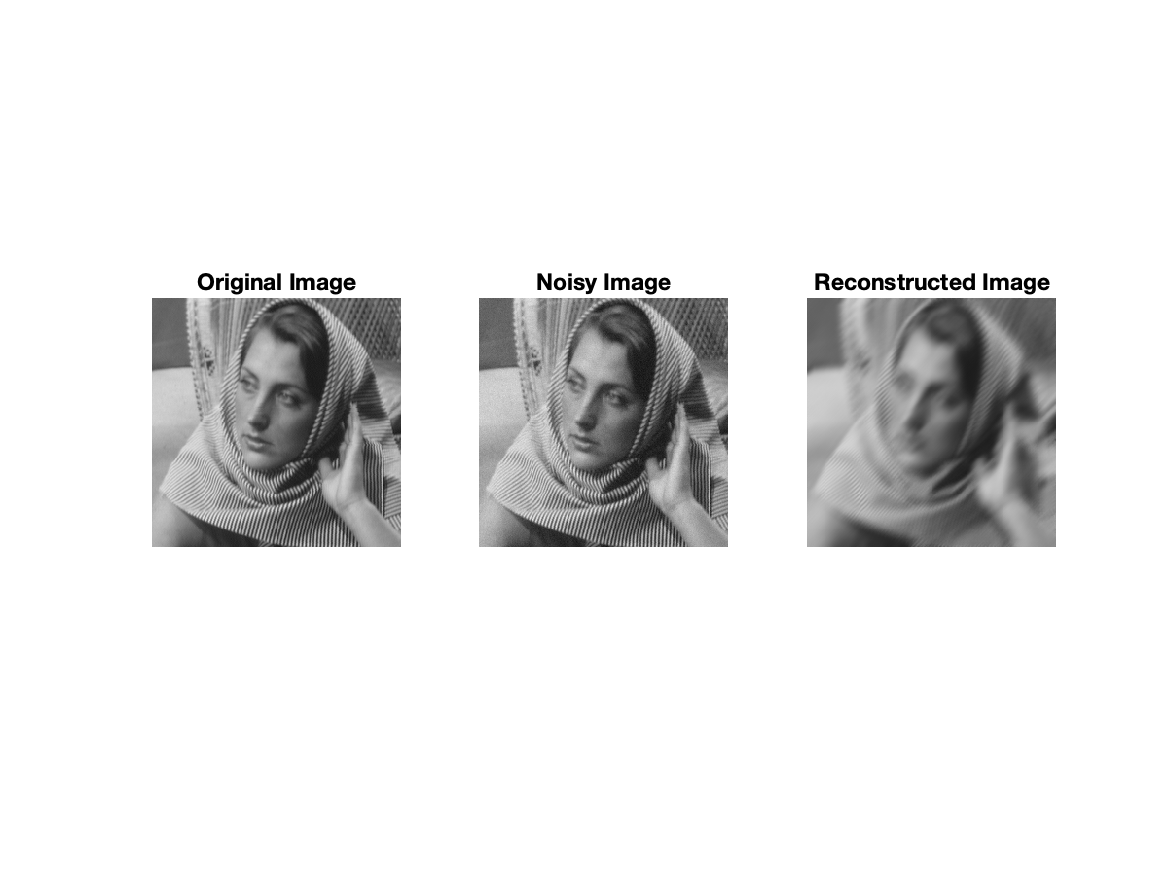
\includegraphics[width=0.5\textwidth]{../FISTA_Barbara.png}
  \caption{ISTA Reconstruction of the Barbara Image}
\end{figure}

\begin{solution}{ISTA Continued}
  The reconstruction does result in a decently accurate recovery of the image. The image is not as sharp as the original image but the major features are still visible. We quantise the quality of the reconstruction by measuring the Root Mean Square Error between the Original Image and the Reconstructed Image. The RMSE value is calculated as :

  \begin{equation}
    \text{RMSE} = \displaystyle\frac{\|X(:) - \hat{X}(:)\|}{\|X(:)\|_2}
  \end{equation}

  \noindent From the above formula, the RMSE value calculated for the ISTA reconstruction of the Barbara Image is \textbf{0.14027}. This value indicates that the reconstruction is quite accurate and the image is well recovered. While increasing the number of iterations and tuning the regularization parameter $\lambda$ can improve the quality of the reconstruction, the current reconstruction is good.

  \noindent Next, we replicate the result on the top left $256 \times 256$ patch of the \textbf{Goldhill Image}. The visual reconstruction of this image is slightly better as evident from the RMSE value of \textbf{0.088862}. The image results are shown below.
\end{solution}

\begin{figure}[!htbp]
  \centering
  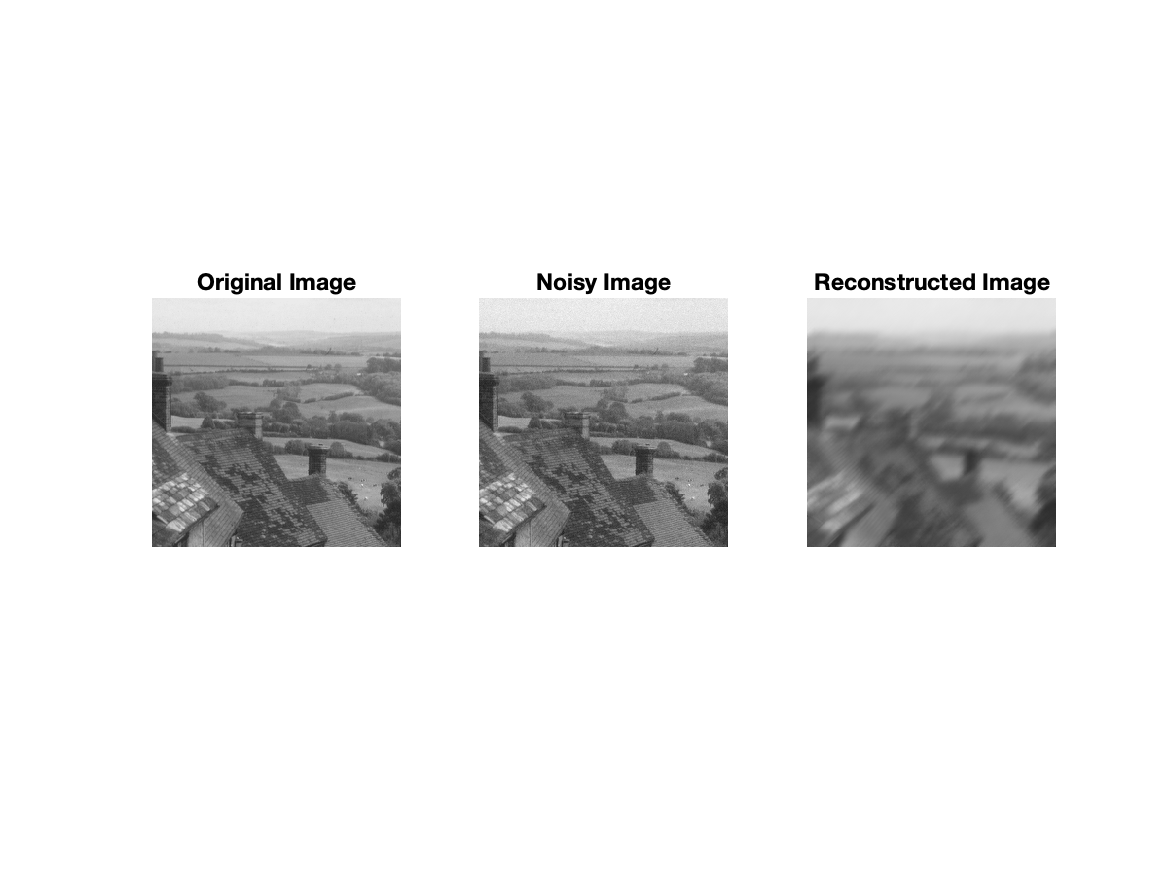
\includegraphics[width=0.5\textwidth]{../ISTA_Goldhill.png}
  \caption{ISTA Reconstruction of the Goldhill Image}
\end{figure}

% 0.14065 0.087743
\begin{solution}{Implementation if FISTA}
  After implementing the ISTA algorithm, we implement the Fast Iterative Soft Thresholding Algorithm (FISTA) for solving the LASSO problem. The FISTA algorithm is an accelerated version of the ISTA algorithm and is given by the following update rules:
  \begin{align}
    x_k &= \text{Soft}(y_k - \alpha A^T(Ay_k - b), \lambda \alpha) \\
    y_{k+1} &= x_k + \frac{t_k-1}{t_k+2} (x_k - x_{k-1}) \\
    t_{k+1} &= \displaystyle\frac{1 + \sqrt{1 + 4t_k^2}}{2}
  \end{align}

  \noindent We implement this update rule for the FISTA algorithm and run the algorithm on the same images as before. The results are shown below. The RMSE values for the Barbara and Goldhill images are \textbf{0.14065} and \textbf{0.087743} respectively. The RMSE values are slightly better than the ISTA algorithm and the visual reconstruction is also better. The images are shown below. This means that the FISTA algorithm is faster than the ISTA algorithm and converges to a better solution in the same number of iterations.

\end{solution}

\begin{figure}[!htbp]
  \centering
  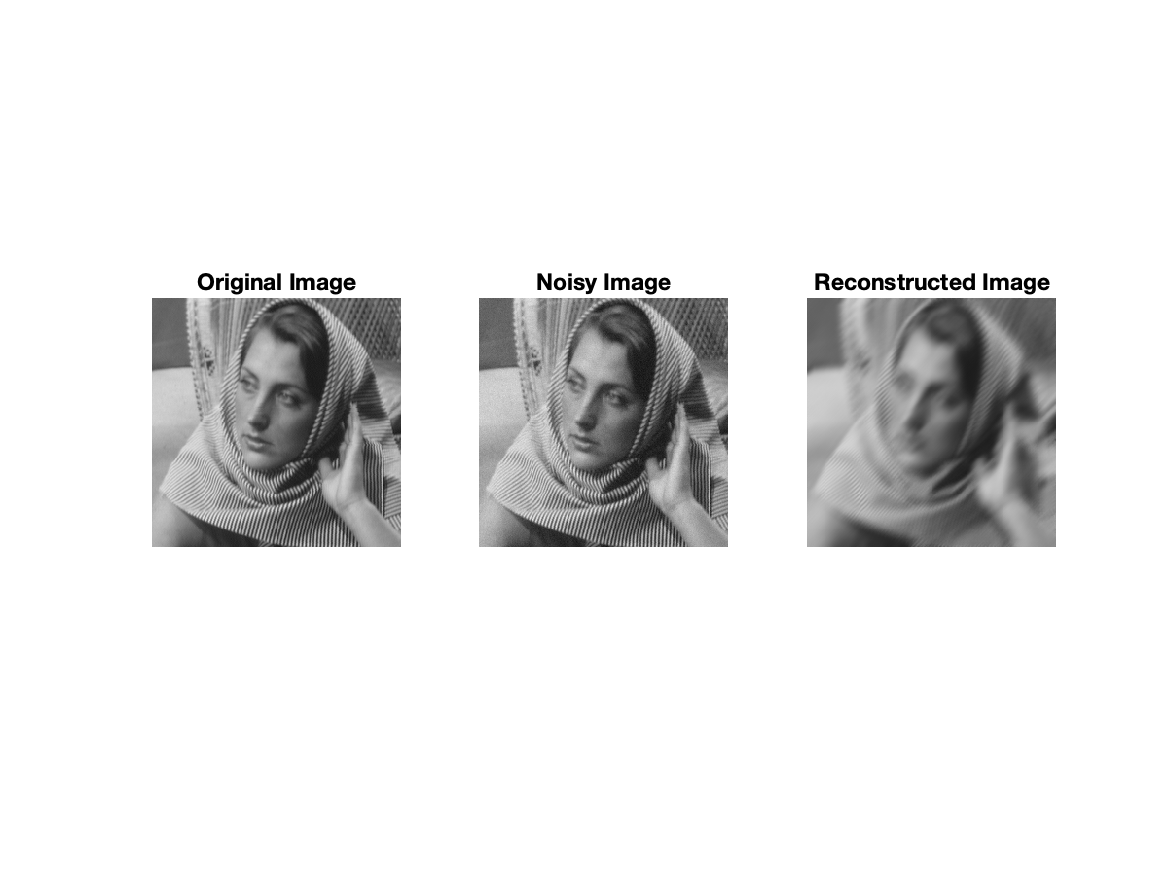
\includegraphics[width=0.5\textwidth]{../FISTA_Barbara.png}
  \caption{FISTA Reconstruction of the Barbara Image}
\end{figure}

\begin{figure}[!htbp]
  \centering
  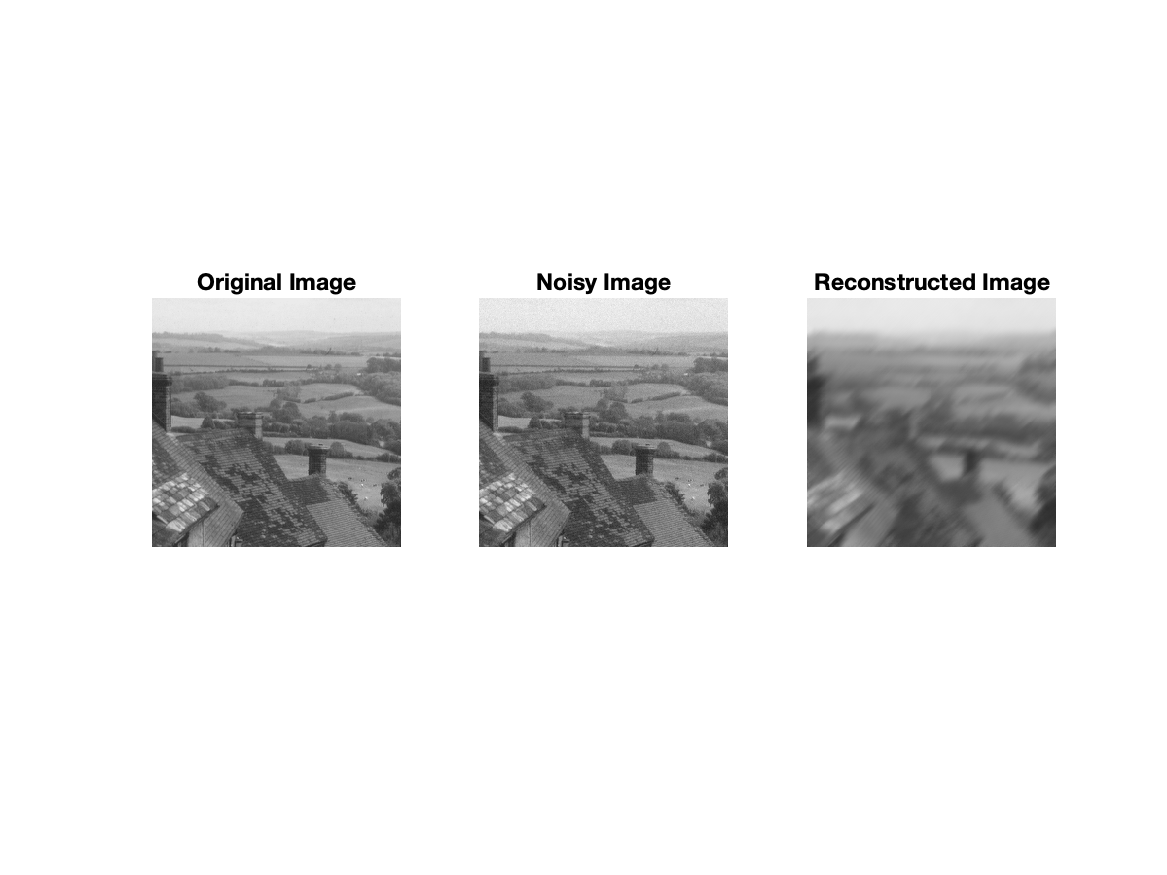
\includegraphics[width=0.5\textwidth]{../FISTA_Goldhill.png}
  \caption{FISTA Reconstruction of the Goldhill Image}
\end{figure}


\begin{solution}{Comparison of ISTA and FISTA}
  \subsection{Convergence of ISTA and FISTA}
  ISTA follows the gradient descent for the soft-thresholding operator. The convergence rate of the ISTA algorithm is sublinear and the decrease in the objective function's value follows the order:
  \begin{equation}
    F(x_k) = F(x^*) \leq \displaystyle\frac{\alpha L(f)\|x_0 - x^*\|^2}{2k}
  \end{equation}
  \noindent Here $\alpha$ is a constant, L(f) is the Lipschitz constant of the gradient of the objective function and $x^*$ is the optimal solution. The resultant convergence rate is $\mathcal{O}(1/k)$, which is slow and requires a large number of iterations to converge to the optimal solution.

  \noindent FISTA, on the other hand accelerates its convergence by incorporating a momentum term. The term is computed based off of both the present and the previous iterates, leading to a faster convergence rate. The global convergece rate of the FISTA algorithm is given by:
  \begin{equation}
    F(x_k) = F(x^*) \leq \displaystyle\frac{2\|x_0 - x^*\|^2}{(k+1)^2}
  \end{equation}
  \noindent The convergence rate of the FISTA algorithm is $\mathcal{O}(1/k^2)$, which is faster than the ISTA algorithm. This is why the FISTA algorithm converges faster than the ISTA algorithm and provides a better reconstruction in the same number of iterations.

  \subsection{Why is FISTA faster than ISTA?}
  The key reason FISTA outperforms ISTA is because of the momentum like step which combines the information from the previous iterates. This allows the algorithm to take larger and more effective steps towards the optimal solution. The core idea of the algorithm is inspired by Nesterov's optimal gradient method. The update rule for FISTA is:
  \begin{equation}
    x_k = p_L(y_k), \quad y_{k + 1} = x_k + \left( \displaystyle\frac{t_k - 1}{t_k + 2}\right) (x_k - x_{k-1})
  \end{equation}
  \noindent Here $p_L$ is the proximal operator associated with the objective function and $t_k$ is the momentum term. The momentum term is updated as:
  \begin{equation}
    t_{k+1} = \displaystyle\frac{1 + \sqrt{1 + 4t_k^2}}{2}
  \end{equation}
  \noindent The convergence of FISTA is established by proving that the function approaches the optimal value at a rate of $\mathcal{O}(1/k^2)$. This is why FISTA is faster than ISTA and provides a better reconstruction in the same number of iterations.

  \noindent \textbf{Lemma : Recursion in FISTA} : The sequence of values generated by the FISTA algorithm satisfy the following inequality:
  \begin{equation}
    \frac{2}{L} \left( t_k^2 F(x_k) - t_{k+1}^2 F(x_{k+1}) \right) \geq \| u_{k+1} \|^2 - \| u_k \|^2
  \end{equation}
  \noindent where \( u_k = t_k x_k - t_{k-1} x_{k-1} - x^*\). This lemma and the smoothness of the objective function are used to prove the convergence of the FISTA algorithm. While both problems use similar update rules, the momentum term in FISTA makes it a much faster algorithm especially for large scale problems.
\end{solution}






\end{document}
